% Unit 118 English translation of chapter8.tex lines 1850--1999.
% Source: Methods of Algebra, Volume 2, commit
% 9a5803ff77dd3257484cb177f851a73770a59dd3 (CC BY 4.0).
% stable-unit-id: o014.aljabr2.chapter8.mapping-cone-revisited
% Coverage: all of Section 8.10, ending immediately before the Exercises.
% Necessary source corrections: line 1855 f(x)->F(x); line 1957
% -f[-1]->-\phi[-1].

% segment-id: o014.li2.chapter8.mapping-cone-revisited.h001
\section{The Mapping Cone Revisited}\label{sec:mapping-cone-revisited}
\hypertarget{o014.aljabr2.chapter8.mapping-cone-revisited}{ }
% segment-id: o014.li2.chapter8.mapping-cone-revisited.p001
As we saw in \S\ref{sec:mapping-cone} and \S\ref{sec:derived-cat}, the
mapping cone $\Cone(f)$ plays an important role in the theory of complexes
and in the study of derived categories. The aim of this section is to
interpret it through the Dold--Kan correspondence and to explain why a
mapping cone really is a ``cone.'' More precisely, we shall study the chain
complex version of the mapping cone; see Remark~\ref{rem:cone-chain}.

% segment-id: o014.li2.chapter8.mapping-cone-revisited.p002
We begin with mapping cones and mapping cylinders in topology. Consider a
continuous map $F:\mathcal{X}\to\mathcal{Y}$ with
$\mathcal{X}\neq\emptyset$. Its mapping cylinder is the quotient space
% segment-id: o014.li2.chapter8.mapping-cone-revisited.q001
\begin{equation*}
	\Cyl_{\mathrm{top}}(F) := \dfrac{(\mathcal{X} \times [0, 1]) \sqcup \mathcal{Y}}{\forall x \in \mathcal{X}, \; (x, 1) \sim F(x)},
\end{equation*}
where $\times$ (respectively, $\sqcup$) denotes the product (respectively,
disjoint union) of topological spaces. The mapping cone is defined by
% segment-id: o014.li2.chapter8.mapping-cone-revisited.q002
\begin{equation*}\begin{aligned}
	\Cone_{\mathrm{top}}(F) & := \dfrac{(\mathcal{X} \times [0, 1]) \sqcup \mathcal{Y}}{\forall x \in \mathcal{X}, \; (x, 1) \sim F(x), \; (x, 0) \sim (\star, 0)} \\
	& \simeq \dfrac{\Cyl_{\mathrm{top}}(F)}{\forall x \in \mathcal{X}, \; (x, 0) \sim (\star, 0)},
\end{aligned}\end{equation*}
where $\star\in\mathcal{X}$ is an arbitrary point. Intuitively,
$\mathcal{X}\times[0,1]$ may be pictured as a tube with cross-section
$\mathcal{X}$. The cylinder $\Cyl_{\mathrm{top}}(F)$ is obtained by gluing
the end $\mathcal{X}\times\{1\}$ of the tube to $\mathcal{Y}$ via $F$,
while $\Cone_{\mathrm{top}}(F)$ further contracts the end
$\mathcal{X}\times\{0\}$ to a single point. Schematically:

% segment-id: o014.li2.chapter8.mapping-cone-revisited.q003
\[ \Cyl_{\mathrm{top}}(F) = 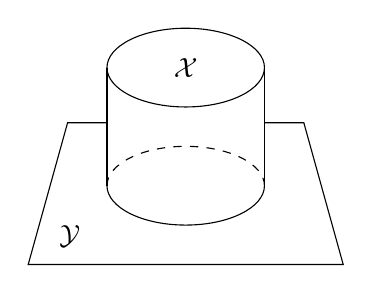
\begin{tikzpicture}[baseline=(O)]
	\draw (1, 1.5) ellipse[x radius=1, y radius=0.5] node {$\mathcal{X}$};
	\draw (0, 0) arc[start angle=180, end angle=360, x radius=1, y radius=0.5];
	\draw[dashed] (0, 0) arc[start angle=180, end angle=0, x radius=1, y radius=0.5];
	\draw (2, 1.5) -- (2, 0);
	\draw (0, 1.5) -- (0, 0);
	\draw (0, 0.8) -- (-0.5, 0.8) -- (-1, -1) node[xshift=1.5em,  yshift=1em] {$\mathcal{Y}$} -- (3, -1) -- (2.5, 0.8) -- (2, 0.8);
	\coordinate (O) at (0, 0.5);
\end{tikzpicture} \quad
	\Cone_{\mathrm{top}}(F) = 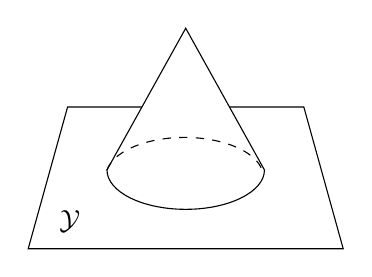
\begin{tikzpicture}[baseline=(O)]
	\draw (0, 0.8) -- (-0.5, 0.8) -- (-1, -1) node[xshift=1.5em,  yshift=1em] {$\mathcal{Y}$} -- (3, -1) -- (2.5, 0.8) --cycle;
	\filldraw[fill=white] (1, 1.8) -- (0, 0) arc[start angle=180, end angle=360, x radius=1, y radius=0.5] --cycle;
	\draw[dashed] (0, 0) arc[start angle=170, end angle=10, x radius=1, y radius=0.5];
	\coordinate (O) at (0, 0.5);
\end{tikzpicture}\]

% segment-id: o014.li2.chapter8.mapping-cone-revisited.p003
Simplicial sets provide a concrete way to describe topological spaces. More
precisely, Theorem~\ref{prop:geom-Sing-adjunction} gives an adjoint pair
% segment-id: o014.li2.chapter8.mapping-cone-revisited.q004
\[\begin{tikzcd}
	{|\cdot|}: \cate{sSet} \arrow[shift left, r] & \cate{Top}: \mathrm{Sing}, \arrow[shift left, l]
\end{tikzcd}\]
and the two categories model equivalent homotopy theories in a precise
sense. The same construction works with $\cate{Top}$ replaced by
$\cate{CGHaus}$. We now translate the preceding discussion into
$\cate{sSet}$. We may assume that
% segment-id: o014.li2.chapter8.mapping-cone-revisited.q005
\[ \mathcal{X} = |X|, \quad \mathcal{Y} = |Y|, \quad F = |f|: |X| \to |Y|, \]
where $f:X\to Y$ is a morphism in $\cate{sSet}$. From the viewpoint of
simplicial sets, the mapping cone is easier to describe than the mapping
cylinder. We begin with the cone on $\mathcal{X}$,
$\Cone_{\mathrm{top}}(\mathcal{X}):=
\Cone_{\mathrm{top}}(\identity_{\mathcal{X}})$. If
$\mathcal{X}=|X|$, then
$\Cone_{\mathrm{top}}(\mathcal{X})\simeq|X^{\lhd}|\simeq|X^{\rhd}|$
(Example~\ref{eg:cone-realization}). Below we focus on the left cone
$X^{\lhd}=\Delta^0\star X$ and its corresponding chain complex.
\index{simplicial set!cone}

% segment-id: o014.li2.chapter8.mapping-cone-revisited.p004
For every simplicial set $Z$, write $Z_n^{\mathrm{nd}}$ for the set of all
nondegenerate $n$-simplices in it, and write
$\{\mathrm{pt}\}=(\Delta^0)_0=(\Delta^0)_0^{\mathrm{nd}}$.
Proposition~\ref{prop:join-nd}, or topological intuition, gives
% segment-id: o014.li2.chapter8.mapping-cone-revisited.q006
\begin{equation}\label{eqn:Cone-X-aux1}
	(\Delta^0 \star X)^{\mathrm{nd}}_n = \begin{cases}
		X^{\mathrm{nd}}_n \sqcup \left( \{ \mathrm{pt} \} \times X^{\mathrm{nd}}_{n-1} \right), & n > 0 \\
		\{\mathrm{pt}\} \sqcup X_0, & n = 0.
	\end{cases}
\end{equation}

% segment-id: o014.li2.chapter8.mapping-cone-revisited.p005
Substituting \eqref{eqn:join-formulas} and the general formulas discussed
above it shows that, for $n\geq1$, the restrictions of
$d_i:(\Delta^0\star X)_n\to(\Delta^0\star X)_{n-1}$ to
$\{\mathrm{pt}\}\times X_{n-1}$ and $X_n$ are as follows:
% segment-id: o014.li2.chapter8.mapping-cone-revisited.q007
\begin{equation}\label{eqn:Cone-X-aux2}\begin{gathered}
	\begin{tikzcd}[column sep=small,
		/tikz/execute at end picture={
			\node [rectangle, draw, fit=(A) (B)] {};
			\node at ($(A)!.5!(C) + (0, 0.8)$) {$1 \leq i \leq n$};
		}]
		|[alias=A]| \{\mathrm{pt}\} \times X_{n-1} \arrow[d, "{\identity \times d_{i-1}}"'] & |[alias=C]| X_n \arrow[d, "{d_i}"] \\
		\{\mathrm{pt}\} \times X_{n-2} & |[alias=B]| X_{n-1}
	\end{tikzcd} \quad
	\begin{tikzcd}[column sep=small,
		/tikz/execute at end picture={
			\node [rectangle, draw, fit=(A) (B)] {};
			\node at ($(A)!.5!(C) + (0, 0.8)$) {$i=0$};
		}]
		|[alias=A]| \{\mathrm{pt}\} \times X_{n-1} \arrow[rd, "{\mathrm{pr}_2}"] & |[alias=C]| X_n \arrow[d, "{d_0}"] \\
		\{\mathrm{pt}\} \times X_{n-2} & |[alias=B]| X_{n-1}
	\end{tikzcd}
\end{gathered}\end{equation}
If $n=1$, the term $\{\mathrm{pt}\}\times X_{n-2}$ in this formula is
to be understood as $\{\mathrm{pt}\}$.

% segment-id: o014.li2.chapter8.mapping-cone-revisited.p006
Since our goal is a chain complex, the next step is to linearize the problem
using the functor $\Z(\mathord\cdot)$ of
Definition~\ref{def:free-simplicial-Ab}, and then pass to chain complexes via
the Dold--Kan correspondence:
% segment-id: o014.li2.chapter8.mapping-cone-revisited.q008
\begin{equation*}
	\mathrm{N}(\Z X^{\lhd}) \simeq \mathrm{C}(\Z X^{\lhd}) \big/ \text{degenerate part} \quad \text{(Proposition \ref{prop:Dold-Kan-v})}.
\end{equation*}
To simplify notation in the rest of this section, write
$\mathrm{N}X:=\mathrm{N}(\Z X)$ and
$\mathrm{N}f:=\mathrm{N}(\Z f)$. The chain-complex structure on
$\mathrm{C}(\Z X^{\lhd})$ comes from
$\partial_n:=\sum_{i=0}^n(-1)^id_i$. Combining
\eqref{eqn:Cone-X-aux1}, \eqref{eqn:Cone-X-aux2}, and the description of
$\Cone(\identity_{\mathrm{N}X})$ in Remark~\ref{rem:cone-chain}, we obtain a
short exact sequence of chain complexes
% segment-id: o014.li2.chapter8.mapping-cone-revisited.q009
\[ 0 \to \underbracket{\Z\{\mathrm{pt}\}}_{\text{degree zero}} \to \mathrm{N}(\Z X^{\lhd}) \to \Cone(\identity_{\mathrm{N}X}) \to 0. \]

% segment-id: o014.li2.chapter8.mapping-cone-revisited.p007
Next, the functors $|\mathord\cdot|$ and
$\mathrm{N}\Z(\mathord\cdot)$ preserve pushout diagrams: the former is a
left adjoint, while the latter is the composite of a left adjoint with an
equivalence; in topology, a pushout diagram means gluing. Therefore, for
$f:X\to Y$ define
% segment-id: o014.li2.chapter8.mapping-cone-revisited.q010
\begin{equation*}
	\Cone_{\mathrm{s}}(f) := X^{\lhd} \dsqcup{X, f} Y.
\end{equation*}
We then obtain
% segment-id: o014.li2.chapter8.mapping-cone-revisited.q011
\[\begin{tikzcd}
	\mathcal{X} \arrow[d, "F"'] \arrow[r, "{\text{base}}"] & \Cone_{\mathrm{top}}(\mathcal{X}) \arrow[d] \\
	\mathcal{Y} \arrow[r] & \Cone_{\mathrm{top}}(F) \arrow[phantom, lu, "\boxplus" description]
\end{tikzcd} \xleftarrow{|\cdot|} \begin{tikzcd}
	X \arrow[d, "f"'] \arrow[r, "\text{canonical}"] & X^{\lhd} \arrow[d] \\
	Y \arrow[r] & \Cone_{\mathrm{s}}(f) \arrow[phantom, lu, "\boxplus" description]
\end{tikzcd} \xrightarrow{\mathrm{N}} \begin{tikzcd}
	\mathrm{N}X \arrow[d, "{\mathrm{N}f}"'] \arrow[r] & \mathrm{N}X^{\lhd} \arrow[d] \\
	\mathrm{N}Y \arrow[r] & \mathrm{N}\Cone_{\mathrm{s}}(f) \arrow[phantom, lu, "\boxplus" description]
\end{tikzcd}\]
This chain of constructions shows that the linear-algebraic counterpart of
$\Cone_{\mathrm{top}}(F)$ should be $\mathrm{N}\Cone_{\mathrm{s}}(f)$.

% segment-id: o014.li2.chapter8.mapping-cone-revisited.pr001
\begin{proposition}\label{prop:Cone-comparison}
	\index{mapping cone}
	With the notation above, there is a canonical short exact sequence of
	chain complexes
	% segment-id: o014.li2.chapter8.mapping-cone-revisited.q012
	\[ 0 \to \underbracket{\Z\{\mathrm{pt}\}}_{\text{degree zero}} \to \mathrm{N}\Cone_{\mathrm{s}}(f) \to \Cone(\mathrm{N}f) \to 0. \]
\end{proposition}
\begin{proof}
	The pushout does not affect the chain subcomplex $\Z\{\mathrm{pt}\}$ of
	$\mathrm{N}X^{\lhd}$ corresponding to the cone point. In degree $n$, it
	replaces every $X_n$ by $Y_n$ and replaces the projection
	$\mathrm{pr}_2$ in \eqref{eqn:Cone-X-aux2} by
	$f_{n-1}\mathrm{pr}_2$. Thus, on the quotient
	$\Cone(\identity_{\mathrm{N}X})$, the resulting pushout is precisely
	$\Cone(\mathrm{N}f)$; see Remark~\ref{rem:cone-chain}.
\end{proof}

% segment-id: o014.li2.chapter8.mapping-cone-revisited.r001
\begin{remark}
	The mapping cylinder $\Cyl_{\mathrm{top}}(F)$ and its chain-complex
	version can be compared similarly; here there is no need to quotient out
	the contribution of the cone point. However, the mapping cylinder involves
	products of simplicial sets, whereas $\mathrm{N}$ is not a monoidal
	functor. Topological accounts therefore usually use CW complexes rather
	than simplicial sets, since products are easier to handle in the world of
	CW complexes.
\end{remark}

% segment-id: o014.li2.chapter8.mapping-cone-revisited.p008
In short, the mapping cone of chain complexes is the quotient of the mapping
cone arising from simplicial sets (or topology) by a copy of $\Z$ coming
from the cone point $\mathrm{pt}$. In the study of chain complexes, the main
role of the mapping cone is that every map $\phi:A\to B$ extends to a
sequence
% segment-id: o014.li2.chapter8.mapping-cone-revisited.q013
\begin{equation}\label{eqn:cofiber-comparison-A}
	A \xrightarrow{\phi} B \to \Cone(\phi) \to A[-1] \xrightarrow{-\phi[-1]} B[-1] \to \cdots .
\end{equation}

% segment-id: o014.li2.chapter8.mapping-cone-revisited.p009
In the topological setting, the map corresponding to
$\Cone(\phi)\to A[-1]$ is obtained by contracting the base
$\mathcal{Y}$ of $\Cone_{\mathrm{top}}(F)$ to a point. The result is denoted
by $S\mathcal{X}$; it is independent of $\mathcal{Y}$ (see the figure below)
and defines a functor $S$. The corresponding sequence of maps is
% segment-id: o014.li2.chapter8.mapping-cone-revisited.q014
\begin{equation*}
	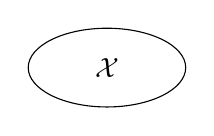
\begin{tikzpicture}[baseline=(O)]
		\draw (1, 0) ellipse[x radius=1, y radius=0.5] node {$\mathcal{X}$};
		\coordinate (O) at (0, 0);
	\end{tikzpicture}
	\xrightarrow{F}
	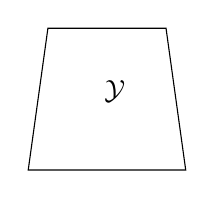
\begin{tikzpicture}[baseline=(O), xscale=0.5]
		\draw (0, 0.8) -- (-0.5, 0.8) -- (-1, -1) -- (3, -1) -- (2.5, 0.8) --cycle;
		\node at (1.2, 0) {$\mathcal{Y}$};
		\coordinate (O) at (0, 0.5);
	\end{tikzpicture}
	\xrightarrow{\text{inclusion}}
	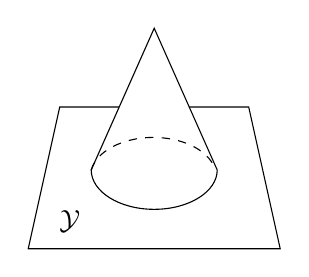
\begin{tikzpicture}[baseline=(O), xscale=0.8]
		\draw (0, 0.8) -- (-0.5, 0.8) -- (-1, -1) node[xshift=1.5em,  yshift=1em] {$\mathcal{Y}$} -- (3, -1) -- (2.5, 0.8) --cycle;
		\filldraw[fill=white] (1, 1.8) -- (0, 0) arc[start angle=180, end angle=360, x radius=1, y radius=0.5] --cycle;
		\draw[dashed] (0, 0) arc[start angle=170, end angle=10, x radius=1, y radius=0.5];
		\coordinate (O) at (0, 0.5);
	\end{tikzpicture}
	\xrightarrow{\text{collapse}}
	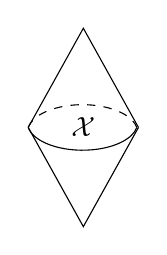
\begin{tikzpicture}[baseline=(O), xscale=0.7, yscale=0.7]
		\draw (2, 0) -- (1, 1.8) -- (0, 0);
		\draw[dashed] (0, 0) arc[start angle=170, end angle=10, x radius=1, y radius=0.5];
		\draw (0, 0) arc[start angle=190, end angle=350, x radius=1, y radius=0.5];
		\node at (1, 0) {$\mathcal{X}$};
		\draw (0, 0) -- (1, -1.8) -- (2, 0);
		\coordinate (O) at (0, 0.5);
	\end{tikzpicture}
	\to \cdots .
\end{equation*}
This sequence is called the \emph{cofiber sequence} generated by $f$ (more
precisely, the unpointed version). If we work in $\cate{sSet}$ and take the
chain complexes of the corresponding sequence, the result is roughly
\eqref{eqn:cofiber-comparison-A}. The qualification ``roughly'' is needed
because:
\begin{itemize}
	\item The map $S\mathcal{X}\to S\mathcal{Y}$ cannot simply be defined as
	$S(F)$; the vertical coordinate must be reversed appropriately. At the
	level of linear algebra, this corresponds to $-\phi[-1]$ in
	\eqref{eqn:cofiber-comparison-A}; see a topology textbook for details.
	\item As Proposition~\ref{prop:Cone-comparison} shows, the various chain
	complexes contain one extra copy of $\Z$ corresponding to the cone point
	of spaces such as $\Cone_{\mathrm{top}}(F)$ and $S\mathcal{X}$. In
	topology, this issue is avoided by using pointed spaces and, in the
	topological cone construction, contracting the part associated with the
	base point.
\end{itemize}

% segment-id: o014.li2.chapter8.mapping-cone-revisited.p010
If we set all details aside for the moment, the theory of derived categories
constructed in \S\ref{sec:derived-cat}, with $\mathcal{A}=\cate{Ab}$, may
also be viewed in broad outline as a somewhat coarse ``linearization'' of
homotopy theory\footnote{More precisely, stable homotopy theory, since chain
complexes allow terms in negative degrees.}.

% segment-id: o014.li2.chapter8.mapping-cone-revisited.p011
As the related questions increasingly involve topological ideas and methods,
we stop here so as not to stray too far afield.
